%
% Copyright (c) 2008, TechnoPark Corp., Florida, USA
% All rights reserved. THIS IS PRIVATE DOCUMENTATION.
%
% Redistribution and use in source and binary forms, with or without modification, are PROHIBITED
% without prior written permission from the author. This product may NOT be used anywhere
% and on any computer except the server platform of TechnoPark Corp. located at
% www.technoparkcorp.com. If you received this code occacionally and without intent to use
% it, please report this incident to the author email: privacy@technoparkcorp.com or
% 470, 555 Bryant St, Palo Alto, CA 94301, the United States of America,
% tel. +1 (860) 506 5536.
%
% @version $Id$
%
\documentclass[12pt,letterpaper,oneside]{article}
\usepackage[T1]{fontenc} % to enable extra symbols
\usepackage[hyperfootnotes=true,unicode]{hyperref}
    \newcommand{\theTitle}{eXtremely Distributed Software Development (XDSD), White Paper}
    \hypersetup{
        unicode=false,
        pdftoolbar=false,
        pdfmenubar=false,
        pdffitwindow=false,
        pdftitle={\theTitle},
        pdfauthor={TechnoPark Corp.},
        pdfsubject={\theTitle},
        pdfnewwindow=true,
        colorlinks=true,
        linkcolor=tpcBlue,
        citecolor=tpcBlue,
        filecolor=tpcBlue,
        urlcolor=tpcBlue
    }
\usepackage{eurosym} % to enable \eur{} command
\usepackage{graphicx} % to enable \includegraphics
    \DeclareGraphicsExtensions{.pdf,.png,.jpg,.gif}
\usepackage{natbib} % for nicer references formatting
    \def\bibfont{\scriptsize}
    \usepackage{etoolbox}
    \patchcmd{\thebibliography}{\sloppy}{\itemsep 0.1cm \parsep 0pt \sloppy}{}{}
\usepackage{fancyhdr}
    \pagestyle{fancy}
    \fancyhf{}
    \renewcommand{\headrulewidth}{0pt}
    \lfoot{
        \begin{textblock}{12}[0,1](6,15)
            {
            \color{tpcLightGrey}\fontfamily{phv}\selectfont\scriptsize\raggedright
            Page \#\thepage{} of \pageref{LastPage},
            \href{http://www.technoparkcorp.com}{www.technoparkcorp.com} \\
            470, 555 Bryant St, Palo Alto, CA 94301, (860) 506 5536 \\
            \today\\
            }
        \end{textblock}
    }
\usepackage{lastpage}
\usepackage{titlesec}
    \titleformat{\section}{\LARGE\fontfamily{phv}\selectfont\color{tpcBlue}}{\thesection{}.}{1em}{}
    \titlespacing{\section}{0cm}{3ex plus .2ex minus .2ex}{2ex minus .2ex}
    \titleformat{\subsection}{\large\fontfamily{phv}\selectfont\color{tpcBlack}}{\thesubsection{}.}{1em}{}
    \titleformat{\subsubsection}{\bfseries\fontfamily{phv}\selectfont\color{tpcBlue}}{\thesubsubsection{}.}{0.5em}{}
\usepackage{array}
\usepackage{setspace}
    \linespread{1.2}
\usepackage{tikz}
	\usetikzlibrary{shapes}
	\usetikzlibrary{arrows}
	\usetikzlibrary{shadows}
	\usetikzlibrary{trees}
	\usetikzlibrary{fit}
	\usetikzlibrary{calc}
	\usetikzlibrary{positioning}
	\usetikzlibrary{decorations.pathmorphing}
    \newcommand{\theTPCLogo}[1]{\begin{tikzpicture}[scale=#1]\path [fill=tpcBlue] (30.019,-26.675) circle (4.753);\path [fill=tpcBlack] (51.953,-15.721) circle (4.753);\path [fill=tpcBlack] (30.022,-15.721) circle (4.753);	\path [fill=tpcBlack] (51.953,-26.675) circle (4.753);	\path [fill=tpcBlack] (51.953,-4.755) circle (4.753);	\path [fill=tpcBlack] (40.982,-4.755) circle (4.753);\path [fill=tpcBlack] (30.022,-4.755) circle (4.753);\path [fill=tpcBlack] (40.982,-15.721) circle (4.753);\path [fill=tpcBlack] (40.982,-26.675) circle (4.753);\path[fill=tpcBlue] (6.037, -31.171)-- (6.037, -31.171) .. controls (5.261, -31.366) and (4.349, -31.495) .. (3.556, -31.495)-- (3.556, -31.495) .. controls (1.952, -31.495) and (1.025, -30.879) .. (1.025, -29.276)-- (1.025, -23.557)-- (0.096, -23.557)-- (0.096, -22.067)-- (1.227, -22.067)-- (1.728, -19.734)-- (3.758, -19.734)-- (3.758, -22.067)-- (5.886, -22.067)-- (5.886, -23.557)-- (3.758, -23.557)-- (3.758, -28.886)-- (3.758, -28.886) .. controls (3.758, -29.615) and (3.878, -30.004) .. (4.654, -30.004)-- (4.654, -30.004) .. controls (5.161, -30.004) and (5.616, -29.68) .. (6.038, -29.566)-- (6.038, -31.171);\path[fill=tpcBlue] (8.597, -23.427)-- (8.597, -23.427) .. controls (9.39, -22.439) and (10.201, -21.937) .. (11.585, -21.937)-- (11.585, -21.937) .. controls (14.302, -21.937) and (15.011, -24.027) .. (15.011, -26.537)-- (15.011, -26.537) .. controls (15.011, -29.453) and (13.626, -31.446) .. (10.47, -31.446)-- (10.47, -31.446) .. controls (10.015, -31.446) and (9.543, -31.397) .. (9.272, -31.349)-- (9.272, -34.006)-- (6.555, -34.006)-- (6.555, -22.067)-- (8.417, -22.067)-- (8.597, -23.427);\path [fill=white](9.271, -29.827)-- (9.271, -29.827) .. controls (9.559, -29.923) and (9.897, -29.956) .. (10.267, -29.956)-- (10.267, -29.956) .. controls (11.99, -29.956) and (12.225, -28.287) .. (12.225, -26.505)-- (12.225, -26.505) .. controls (12.225, -24.918) and (11.972, -23.427) .. (10.79, -23.427)-- (10.79, -23.427) .. controls (9.373, -23.427) and (9.27, -24.918) .. (9.27, -26.295)-- (9.27, -29.827);\path[fill=tpcBlue] (22.076, -31.252)-- (22.076, -31.252) .. controls (21.368, -31.415) and (20.659, -31.495) .. (19.866, -31.495)-- (19.866, -31.495) .. controls (16.44, -31.495) and (15.579, -29.211) .. (15.579, -26.619)-- (15.579, -26.619) .. controls (15.579, -23.947) and (16.777, -21.938) .. (20.137, -21.938)-- (20.137, -21.938) .. controls (20.811, -21.938) and (21.351, -21.987) .. (22.082, -22.133)-- (22.082, -23.624)-- (22.082, -23.624) .. controls (21.435, -23.477) and (20.946, -23.428) .. (20.389, -23.428)-- (20.389, -23.428) .. controls (18.701, -23.428) and (18.381, -25.016) .. (18.381, -26.636)-- (18.381, -26.636) .. controls (18.381, -28.466) and (18.701, -30.005) .. (20.405, -30.005)-- (20.405, -30.005) .. controls (20.998, -30.005) and (21.537, -29.958) .. (22.076, -29.828)-- (22.076, -31.252);\path[fill=tpcBlack] (0, -36.638)-- (0, -36.638) .. controls (0.271, -36.593) and (0.624, -36.555) .. (1.075, -36.555)-- (1.075, -36.555) .. controls (1.63, -36.555) and (2.036, -36.684) .. (2.292, -36.915)-- (2.292, -36.915) .. controls (2.531, -37.121) and (2.672, -37.436) .. (2.672, -37.824)-- (2.672, -37.824) .. controls (2.672, -38.216) and (2.557, -38.525) .. (2.338, -38.751)-- (2.338, -38.751) .. controls (2.042, -39.066) and (1.559, -39.228) .. (1.011, -39.228)-- (1.011, -39.228) .. controls (0.844, -39.228) and (0.69, -39.222) .. (0.561, -39.189)-- (0.561, -40.928)-- (0, -40.928)-- (0, -36.638);\path [fill=white](0.561, -38.73)-- (0.561, -38.73) .. controls (0.684, -38.763) and (0.837, -38.775) .. (1.025, -38.775)-- (1.025, -38.775) .. controls (1.701, -38.775) and (2.114, -38.446) .. (2.114, -37.847)-- (2.114, -37.847) .. controls (2.114, -37.274) and (1.707, -36.997) .. (1.089, -36.997)-- (1.089, -36.997) .. controls (0.845, -36.997) and (0.658, -37.016) .. (0.562, -37.042)-- (0.562, -38.73);\path[fill=tpcBlack] (4.019, -36.354)-- (4.585, -36.354)-- (4.585, -40.926)-- (4.019, -40.926)-- (4.019, -36.354);\path[fill=tpcBlack] (8.372, -40.18)-- (8.372, -40.18) .. controls (8.372, -40.451) and (8.385, -40.715) .. (8.423, -40.927)-- (7.908, -40.927)-- (7.863, -40.534)-- (7.843, -40.534)-- (7.843, -40.534) .. controls (7.669, -40.778) and (7.334, -40.997) .. (6.89, -40.997)-- (6.89, -40.997) .. controls (6.26, -40.997) and (5.937, -40.552) .. (5.937, -40.102)-- (5.937, -40.102) .. controls (5.937, -39.349) and (6.607, -38.936) .. (7.811, -38.942)-- (7.811, -38.879)-- (7.811, -38.879) .. controls (7.811, -38.621) and (7.741, -38.157) .. (7.103, -38.157)-- (7.103, -38.157) .. controls (6.813, -38.157) and (6.51, -38.247) .. (6.291, -38.388)-- (6.162, -38.014)-- (6.162, -38.014) .. controls (6.42, -37.847) and (6.794, -37.738) .. (7.185, -37.738)-- (7.185, -37.738) .. controls (8.138, -37.738) and (8.371, -38.388) .. (8.371, -39.013)-- (8.371, -40.18);\path [fill=white](7.824, -39.336)-- (7.824, -39.336) .. controls (7.206, -39.323) and (6.504, -39.433) .. (6.504, -40.038)-- (6.504, -40.038) .. controls (6.504, -40.405) and (6.75, -40.579) .. (7.039, -40.579)-- (7.039, -40.579) .. controls (7.444, -40.579) and (7.702, -40.322) .. (7.793, -40.058)-- (7.793, -40.058) .. controls (7.812, -40) and (7.824, -39.935) .. (7.824, -39.877)-- (7.824, -39.336);\path[fill=tpcBlack] (9.93, -38.653)-- (9.93, -38.653) .. controls (9.93, -38.331) and (9.924, -38.067) .. (9.905, -37.809)-- (10.408, -37.809)-- (10.439, -38.325)-- (10.452, -38.325)-- (10.452, -38.325) .. controls (10.606, -38.029) and (10.969, -37.739) .. (11.483, -37.739)-- (11.483, -37.739) .. controls (11.915, -37.739) and (12.584, -37.996) .. (12.584, -39.065)-- (12.584, -40.926)-- (12.018, -40.926)-- (12.018, -39.13)-- (12.018, -39.13) .. controls (12.018, -38.628) and (11.831, -38.209) .. (11.296, -38.209)-- (11.296, -38.209) .. controls (10.922, -38.209) and (10.633, -38.473) .. (10.537, -38.789)-- (10.537, -38.789) .. controls (10.511, -38.86) and (10.498, -38.957) .. (10.498, -39.054)-- (10.498, -40.928)-- (9.93, -40.928)-- (9.93, -38.653);\path[fill=tpcBlack] (16.847, -40.927)-- (16.847, -39.086)-- (15.476, -36.587)-- (16.114, -36.587)-- (16.724, -37.784)-- (16.724, -37.784) .. controls (16.893, -38.113) and (17.02, -38.377) .. (17.156, -38.68)-- (17.17, -38.68)-- (17.17, -38.68) .. controls (17.291, -38.397) and (17.441, -38.114) .. (17.607, -37.784)-- (18.232, -36.587)-- (18.87, -36.587)-- (17.416, -39.079)-- (17.416, -40.928)-- (16.847, -40.928);\path[fill=tpcBlack] (22.32, -39.342)-- (22.32, -39.342) .. controls (22.32, -40.495) and (21.521, -40.997) .. (20.768, -40.997)-- (20.768, -40.997) .. controls (19.924, -40.997) and (19.274, -40.379) .. (19.274, -39.393)-- (19.274, -39.393) .. controls (19.274, -38.35) and (19.957, -37.738) .. (20.819, -37.738)-- (20.819, -37.738) .. controls (21.715, -37.739) and (22.32, -38.389) .. (22.32, -39.342);\path [fill=white](19.848, -39.375)-- (19.848, -39.375) .. controls (19.848, -40.058) and (20.241, -40.573) .. (20.794, -40.573)-- (20.794, -40.573) .. controls (21.335, -40.573) and (21.741, -40.065) .. (21.741, -39.363)-- (21.741, -39.363) .. controls (21.741, -38.835) and (21.476, -38.165) .. (20.807, -38.165)-- (20.807, -38.165) .. controls (20.137, -38.164) and (19.848, -38.782) .. (19.848, -39.375);\path[fill=tpcBlack] (26.287, -40.077)-- (26.287, -40.077) .. controls (26.287, -40.399) and (26.293, -40.682) .. (26.313, -40.927)-- (25.81, -40.927)-- (25.778, -40.418)-- (25.765, -40.418)-- (25.765, -40.418) .. controls (25.617, -40.669) and (25.287, -40.998) .. (24.734, -40.998)-- (24.734, -40.998) .. controls (24.245, -40.998) and (23.659, -40.727) .. (23.659, -39.633)-- (23.659, -37.81)-- (24.226, -37.81)-- (24.226, -39.537)-- (24.226, -39.537) .. controls (24.226, -40.129) and (24.407, -40.528) .. (24.921, -40.528)-- (24.921, -40.528) .. controls (25.301, -40.528) and (25.565, -40.264) .. (25.667, -40.013)-- (25.667, -40.013) .. controls (25.7, -39.93) and (25.72, -39.826) .. (25.72, -39.723)-- (25.72, -37.81)-- (26.286, -37.81)-- (26.286, -40.077);\path[fill=tpcBlack] (27.871, -38.782)-- (27.871, -38.782) .. controls (27.871, -38.415) and (27.865, -38.099) .. (27.846, -37.809)-- (28.341, -37.809)-- (28.361, -38.421)-- (28.387, -38.421)-- (28.387, -38.421) .. controls (28.529, -38.003) and (28.869, -37.739) .. (29.25, -37.739)-- (29.25, -37.739) .. controls (29.313, -37.739) and (29.359, -37.745) .. (29.41, -37.758)-- (29.41, -38.293)-- (29.41, -38.293) .. controls (29.351, -38.28) and (29.294, -38.274) .. (29.218, -38.274)-- (29.218, -38.274) .. controls (28.819, -38.274) and (28.535, -38.576) .. (28.458, -39.002)-- (28.458, -39.002) .. controls (28.444, -39.079) and (28.432, -39.169) .. (28.432, -39.266)-- (28.432, -40.928)-- (27.871, -40.928)-- (27.871, -38.782);\path[fill=tpcBlack] (32.572, -40.244)-- (32.572, -40.244) .. controls (32.823, -40.398) and (33.189, -40.527) .. (33.576, -40.527)-- (33.576, -40.527) .. controls (34.149, -40.527) and (34.485, -40.224) .. (34.485, -39.786)-- (34.485, -39.786) .. controls (34.485, -39.381) and (34.253, -39.149) .. (33.667, -38.923)-- (33.667, -38.923) .. controls (32.959, -38.672) and (32.521, -38.305) .. (32.521, -37.693)-- (32.521, -37.693) .. controls (32.521, -37.017) and (33.081, -36.514) .. (33.925, -36.514)-- (33.925, -36.514) .. controls (34.369, -36.514) and (34.692, -36.617) .. (34.884, -36.727)-- (34.731, -37.185)-- (34.731, -37.185) .. controls (34.588, -37.107) and (34.298, -36.978) .. (33.907, -36.978)-- (33.907, -36.978) .. controls (33.314, -36.978) and (33.088, -37.332) .. (33.088, -37.628)-- (33.088, -37.628) .. controls (33.088, -38.034) and (33.353, -38.233) .. (33.951, -38.465)-- (33.951, -38.465) .. controls (34.685, -38.749) and (35.058, -39.103) .. (35.058, -39.74)-- (35.058, -39.74) .. controls (35.058, -40.409) and (34.562, -40.996) .. (33.538, -40.996)-- (33.538, -40.996) .. controls (33.12, -40.996) and (32.662, -40.867) .. (32.431, -40.713)-- (32.572, -40.244);\path[fill=tpcBlack] (39.058, -40.077)-- (39.058, -40.077) .. controls (39.058, -40.399) and (39.065, -40.682) .. (39.082, -40.927)-- (38.58, -40.927)-- (38.548, -40.418)-- (38.536, -40.418)-- (38.536, -40.418) .. controls (38.387, -40.669) and (38.059, -40.998) .. (37.505, -40.998)-- (37.505, -40.998) .. controls (37.016, -40.998) and (36.431, -40.727) .. (36.431, -39.633)-- (36.431, -37.81)-- (36.996, -37.81)-- (36.996, -39.537)-- (36.996, -39.537) .. controls (36.996, -40.129) and (37.176, -40.528) .. (37.692, -40.528)-- (37.692, -40.528) .. controls (38.071, -40.528) and (38.336, -40.264) .. (38.438, -40.013)-- (38.438, -40.013) .. controls (38.471, -39.93) and (38.49, -39.826) .. (38.49, -39.723)-- (38.49, -37.81)-- (39.057, -37.81)-- (39.057, -40.077);\path[fill=tpcBlack] (42.863, -40.81)-- (42.863, -40.81) .. controls (42.715, -40.888) and (42.386, -40.998) .. (41.967, -40.998)-- (41.967, -40.998) .. controls (41.028, -40.998) and (40.415, -40.354) .. (40.415, -39.401)-- (40.415, -39.401) .. controls (40.415, -38.441) and (41.071, -37.746) .. (42.089, -37.746)-- (42.089, -37.746) .. controls (42.425, -37.746) and (42.72, -37.829) .. (42.875, -37.907)-- (42.746, -38.345)-- (42.746, -38.345) .. controls (42.61, -38.268) and (42.398, -38.197) .. (42.089, -38.197)-- (42.089, -38.197) .. controls (41.375, -38.197) and (40.987, -38.725) .. (40.987, -39.375)-- (40.987, -39.375) .. controls (40.987, -40.096) and (41.451, -40.541) .. (42.07, -40.541)-- (42.07, -40.541) .. controls (42.39, -40.541) and (42.603, -40.457) .. (42.765, -40.386)-- (42.863, -40.81);\path[fill=tpcBlack] (46.353, -40.81)-- (46.353, -40.81) .. controls (46.206, -40.888) and (45.877, -40.998) .. (45.458, -40.998)-- (45.458, -40.998) .. controls (44.518, -40.998) and (43.906, -40.354) .. (43.906, -39.401)-- (43.906, -39.401) .. controls (43.906, -38.441) and (44.563, -37.746) .. (45.58, -37.746)-- (45.58, -37.746) .. controls (45.915, -37.746) and (46.212, -37.829) .. (46.366, -37.907)-- (46.237, -38.345)-- (46.237, -38.345) .. controls (46.102, -38.268) and (45.889, -38.197) .. (45.58, -38.197)-- (45.58, -38.197) .. controls (44.865, -38.197) and (44.479, -38.725) .. (44.479, -39.375)-- (44.479, -39.375) .. controls (44.479, -40.096) and (44.943, -40.541) .. (45.56, -40.541)-- (45.56, -40.541) .. controls (45.883, -40.541) and (46.095, -40.457) .. (46.256, -40.386)-- (46.353, -40.81);\path[fill=tpcBlack] (47.938, -39.471)-- (47.938, -39.471) .. controls (47.951, -40.238) and (48.441, -40.553) .. (49.006, -40.553)-- (49.006, -40.553) .. controls (49.412, -40.553) and (49.657, -40.483) .. (49.869, -40.392)-- (49.966, -40.798)-- (49.966, -40.798) .. controls (49.766, -40.888) and (49.425, -40.998) .. (48.93, -40.998)-- (48.93, -40.998) .. controls (47.969, -40.998) and (47.397, -40.36) .. (47.397, -39.42)-- (47.397, -39.42) .. controls (47.397, -38.48) and (47.951, -37.739) .. (48.859, -37.739)-- (48.859, -37.739) .. controls (49.877, -37.739) and (50.147, -38.634) .. (50.147, -39.207)-- (50.147, -39.207) .. controls (50.147, -39.323) and (50.133, -39.413) .. (50.126, -39.471)-- (47.938, -39.471);\path [fill=white](49.599, -39.065)-- (49.599, -39.065) .. controls (49.605, -38.705) and (49.451, -38.144) .. (48.813, -38.144)-- (48.813, -38.144) .. controls (48.241, -38.144) and (47.99, -38.672) .. (47.944, -39.065)-- (49.599, -39.065);\path[fill=tpcBlack] (51.415, -40.347)-- (51.415, -40.347) .. controls (51.583, -40.456) and (51.878, -40.572) .. (52.162, -40.572)-- (52.162, -40.572) .. controls (52.574, -40.572) and (52.767, -40.366) .. (52.767, -40.109)-- (52.767, -40.109) .. controls (52.767, -39.838) and (52.605, -39.69) .. (52.187, -39.536)-- (52.187, -39.536) .. controls (51.626, -39.336) and (51.363, -39.027) .. (51.363, -38.653)-- (51.363, -38.653) .. controls (51.363, -38.151) and (51.769, -37.739) .. (52.438, -37.739)-- (52.438, -37.739) .. controls (52.753, -37.739) and (53.03, -37.829) .. (53.204, -37.932)-- (53.063, -38.344)-- (53.063, -38.344) .. controls (52.941, -38.267) and (52.715, -38.164) .. (52.425, -38.164)-- (52.425, -38.164) .. controls (52.09, -38.164) and (51.904, -38.357) .. (51.904, -38.589)-- (51.904, -38.589) .. controls (51.904, -38.846) and (52.09, -38.962) .. (52.496, -39.117)-- (52.496, -39.117) .. controls (53.036, -39.323) and (53.313, -39.594) .. (53.313, -40.057)-- (53.313, -40.057) .. controls (53.313, -40.604) and (52.888, -40.997) .. (52.148, -40.997)-- (52.148, -40.997) .. controls (51.806, -40.997) and (51.491, -40.907) .. (51.272, -40.778)-- (51.415, -40.347);\path[fill=tpcBlack] (54.608, -40.347)-- (54.608, -40.347) .. controls (54.776, -40.456) and (55.072, -40.572) .. (55.355, -40.572)-- (55.355, -40.572) .. controls (55.767, -40.572) and (55.961, -40.366) .. (55.961, -40.109)-- (55.961, -40.109) .. controls (55.961, -39.838) and (55.799, -39.69) .. (55.381, -39.536)-- (55.381, -39.536) .. controls (54.82, -39.336) and (54.556, -39.027) .. (54.556, -38.653)-- (54.556, -38.653) .. controls (54.556, -38.151) and (54.962, -37.739) .. (55.632, -37.739)-- (55.632, -37.739) .. controls (55.947, -37.739) and (56.224, -37.829) .. (56.398, -37.932)-- (56.256, -38.344)-- (56.256, -38.344) .. controls (56.134, -38.267) and (55.908, -38.164) .. (55.619, -38.164)-- (55.619, -38.164) .. controls (55.283, -38.164) and (55.097, -38.357) .. (55.097, -38.589)-- (55.097, -38.589) .. controls (55.097, -38.846) and (55.284, -38.962) .. (55.69, -39.117)-- (55.69, -39.117) .. controls (56.231, -39.323) and (56.508, -39.594) .. (56.508, -40.057)-- (56.508, -40.057) .. controls (56.508, -40.604) and (56.082, -40.997) .. (55.342, -40.997)-- (55.342, -40.997) .. controls (55.001, -40.997) and (54.686, -40.907) .. (54.467, -40.778)-- (54.608, -40.347);\end{tikzpicture}}
\usepackage{xcolor}
    \definecolor{tpcBlue}{rgb}{0,0.5765,0.8196} %
    \definecolor{tpcBlack}{rgb}{0.0863,0.1608,0.2039}
    \definecolor{tpcGrey}{rgb}{0.2706,0.3333,0.3765} %
    \definecolor{tpcLightGrey}{rgb}{0.6784,0.7255,0.7529}
    \definecolor{tpcGreen}{rgb}{0.3294,0.7255,0.2824}
    \definecolor{tpcRed}{rgb}{0.8902,0.1059,0.1373}
    \definecolor{tpcYellow}{rgb}{1,0.9569,0.3294}
    \definecolor{tpcRUPBody}{rgb}{1,1,0.8}
    \definecolor{tpcRUPBorder}{rgb}{0.6039,0,0.2}
    \color{tpcBlack}
\usepackage[absolute]{textpos}
    \TPGrid{16}{16}
\usepackage[top=2.5\TPVertModule, bottom=3\TPVertModule, left=6\TPHorizModule, right=2\TPHorizModule]{geometry}
\usepackage{marginnote} % for nice margin notes
    \reversemarginpar
    \renewcommand*{\marginfont}{\color{tpcBlue}\large}
    \setlength{\marginparsep}{0.5\TPHorizModule}
    \setlength{\marginparwidth}{3\TPHorizModule}
\usepackage[hang,ragged,symbol]{footmisc} % for nice footnotes
    \addtolength{\skip\footins}{4em plus 1em}
\usepackage{wrapfig}
\usepackage{picins} % for wrapping text around objects

% set this font as default
    \renewcommand\familydefault{\sfdefault}
    \renewcommand\sfdefault{phv}
    \normalfont
% don't break pars
    % \interlinepenalty=10000

% for translation
% \usepackage[utf8]{inputenc}
% \usepackage[T2B]{fontenc}
\newcommand{\enru}[2]{#1}

\begin{document}
    \setlength{\parskip}{0.3cm}
    \setlength{\parindent}{0cm}
\raggedright



    \thispagestyle{empty}

    {\fontsize{48pt}{48pt}\color{tpcBlue}\selectfont
        \enru{
            eXtremely\par
            Distributed\par
            Software\par
            Development\par
        }{
            Экстремально\par
            Распределенное\par
            Программирование\par
        }
    }

    \vspace*{5em}
    \colorbox{tpcBlue}{\color{white}white paper}

    \begin{minipage}{20em}\scriptsize\setstretch{1.2}\raggedright
    Some inventions explained in the
    document are protected by the Patent Law of the United States,
    patent applications:
    12/193,010, 12/264,370, 12/703,202, 12/840,306, and 12/943,022.
    \end{minipage}

    \begin{textblock}{3}[1,1](6,15){
        \theTPCLogo{0.05}
    }\end{textblock}

    \begin{textblock}{6}[0,1](6,15){
        TechnoPark Corp.\\
        470, 555 Bryant St, \\
        Palo Alto, CA 94301 \\
        (860) 506 5536
    }\end{textblock}

    \newpage





    \enru{
        In this document we introduce
        eXtremely Distributed Software Development (\href{http://www.xdsd.org}{XDSD})
        methodology
        and explain how it reduces risks and improves quality.
    }
    {
        Настоящий документ представляет
        XDSD (eXtremely Distributed Software Development),
        объясняя, как эта методология снижает
        риски и повышает качество.
    }







\phantomsection
\addcontentsline{toc}{section}{\enru{Are We Getting Any Better?}{Ситуация улучшается?}}
\section*{\enru{Are We Getting Any Better?}{Ситуация улучшается?}}

    \enru{
        Jeff Atwood said in
        \href{http://www.codinghorror.com/blog/2006/05/the-long-dismal-history-of-software-project-failure.html}{his blog}
        four years ago:
        ``The history of software development is a tremendous success.
        Just look around you for evidence of that. But that success
        has a long, dark shadow that we don't talk about very much:
        it's littered with colossal failures. What's particularly disturbing
        is that the colossal failures keep recurring year after year.''
        Sadly, since then we have not been getting much better.
    }{
        Джефф Этвуд сказал с своем блоге четыре года назад:
        ``История развития программирования --- это огромный успех. Только
        посмотрите вокруг и найдете множество свидетельств тому. Но этот
        успех сопряжен с колоссальными неудачами, о которых мы предпочитаем молчать.
        Что особенно неприятно, так это повторение этих неудач из года в год.''
        К сожалению с тех пор ситуация не улучшилась.
    }

    \enru{
        \citet{chaos10}, the latest report by Standish Group based on the analysis
        of 70,000 IT projects,
        shows that the industry ``failure rate'' is over 68\% and is not decreasing.
        \citet{cerpa09} gives a representative summary of other recent studies,
        which mostly agree that software quality is not improving, but getting worse
        every year.
    }{
        Последний отчет Standish Group, основанный на анализе 70-ти тысяч
        проектов показывает, что неуспешных среди них более 68\%,
        и этот показатель не снижается.
        \citet{cerpa09} суммирует последние исследования, которые сходятся
        в одном, --- качество программных продуктов не улучшается, а ухудшается
        каждый год.
    }

    \marginnote{
        ``\enru{Billions of dollars are wasted each year on bad software.}
            {Миллиарды долларов тратятся ежегодно на разработку некачественного ПО}''\\
        \small-- \enru{Bob Charette}{Боб Чаретте}
    }
    \enru{
        \citet{charette05} says that while billions of dollars
        are wasted each year on bad software,
        few IT projects truly succeed.
    }{
        \citet{charette05} отмечает, что миллиарды долларов
        тратятся ежегодно на разработку некачественого программного обеспечения,
        и лишь немногие проекты действительно успешны.
    }

    \enru{
        Is there a bad pattern associated with projects falling short? Do such cases
        look similar to each other? In this white paper, we explore those questions and provide an example of a process that does work.
    }{
        Похожи ли провальные проекты друг на друга и можно
        ли обнаружить единый сценарий этих неудач?
    }







\phantomsection
\addcontentsline{toc}{section}{\enru{How It Happens}{Как это случается?}}
\section*{\enru{How It Happens}{Как это случается?}}

    \enru{
        Imagine that you have a business process based on paper documents, and
        you discover a strong market demand to make them electronic and available over the Internet.
    }{
        Представьте, что Вы собираетесь автоматизировать и компьютеризировать
        существующие бизнес процессы, создав информационную систему предприятия.
    }

    \enru{
        So you find and hire a reputable software development company
        with good references and the readiness to make your project happen
        for a flat fee of \$180 per hour. The developer gives a precise and accurate
        estimate of the project size, equal to 2585 hours, making the total
        project budget equal to \$465,300.
    }{
        Вы находите и нанимаете разработчика информационной системы,
        успешную компанию с многолетней репутацией, готовой выполнить
        работы за \$180 долларов в час. Разработчик оценивает объем
        работы в 2585 часов. Общий бюджет проекта составляет \$465.300.
    }

    \enru{
        In a few months and after a number of payments made to the developer, you see
        a demo version of the product. You like it; however it misses
        a few important features which are critical for the business.
        The developer documents your suggestions and comes up with a new budget.
        You approve it and wait for the next demonstration, which happens in
        a few months.
    }{
        Через несколько месяцев и после нескольких платежей разработчику
        Вы получаете демо-версию продукта. Она выглядит привлекательно,
        однако в ней нехватает ряда важных функций. Разработчик регистрирует
        Ваши пожелания и предлагает на утверждение новые сроки и новый бюджет.
        Вы утверждаете их и ожидаете следующей демонстрации, через несколько
        месяцев.
    }

    \enru{
        After the 13th demonstration and four years of work,
        the budget has increased and \$3.1 million has been paid to the developer.
        The system is still not finished and has not been delivered to your end-users.
    }{
        После 13-й демонстрации и четырех лет работы бюджет проекта
        составляет \$3.1 миллион долларов, большую часть из которых
        Вы уже выплатили. Система пока не запущена в эксплуатацию.
    }

    \enru{
        A reality check reveals that there is no system in place,
        but rather a large amount of messy documentation
        and software components not compatible with each other.
        You hire another vendor to get an independent oversight,
        which reviews the existing artifacts and comes up
        with a new project budget of \$1.8 million, claiming that ``it has to
        be redone from scratch''. However, at this point you are out of time and the budget has run out.
    }{
        После детального анализа созданного продукта Вы понимаете,
        что системы не существует как таковой. Вместо нее Вы
        имеете большой объем документации и несвязанных между собой
        программных модулей. Вы нанимаете нового разработчика, который
        заявляет, что может создать продукт с нуля за \$1.8 миллиона.
        У Вас нет больше времени и средств.
    }

    \marginnote{
        ``\enru{...independent oversight reveals that there is no system in place}
            {...экспертный анализ установил, что системы не существует вовсе}''\\
        \small-- \enru{audit report}{аудиторский отчет}
    }
    \enru{
        Don't be surprised if this story sounds familiar. This is not fiction, but rather a summary of what
        \citet{thompson03}, New York City Controller, documented in his audit of
        a project once outsourced by the NYC Department of Health and Mental Hygiene
        to IBM Corporation.
    }{
        Не удивляйтесь, если это выглядит похоже на то, что происходит
        в Вашем бизнесе. Это не выдуманная история, а выдержка из
        аудиторского отчета, который \citet{thompson03} составил по результатам
        проверки работы компании IBM для департамента здоровья мэрии города Нью-Йорк.
    }

    \enru{
        If IBM, a global corporation, makes such mistakes, how can we avoid them?
        Is it just impossible due
        to the ``essential complexity'' of software?
    }{
        Если IBM совершает подобные ошибки, как мы можем их избежать?
        Может быть это невозможно из-за ``естественной сложности''
        программных продуктов?
    }






\phantomsection
\addcontentsline{toc}{section}{\enru{What History Says}{Что говорит опыт?}}
\section*{\enru{What History Says}{Что говорит опыт?}}

    \enru{
        Since 1960x, when software engineering as an independent profession was born,
        the success factors of software projects concerned their sponsors.
        There were two principles discovered in the industry and emphasized
        by \citet{brooks95}.
        First, there is no ``silver bullet''. Second,
        if a ``silver bullet'' does exist, despite principle
        one, then the solution is a discipline
        (also known as formal methods, process, methodology,
        framework, best practices, etc.).
    }{
        Начиная с 60-х годов, когда ``software engineering'' появилась
        как самостоятельная профессия, многие пытаются найти формулу успеха
        для проектов по разработке
        программного обеспечения. \citet{brooks95}
        высказал две важные мысли. Во-первых, универсальной формулы нет.
        Во-вторых, если она и есть, то это дисциплина, также известная
        как формальная методика, процесс, методология, правила работы и пр.)
    }

    \marginnote{\color{tpcBlack}%
% Copyright (c) 2008, TechnoPark Corp., Florida, USA
% All rights reserved. THIS IS PRIVATE DOCUMENTATION.
%
% Redistribution and use in source and binary forms, with or without modification, are PROHIBITED
% without prior written permission from the author. This product may NOT be used anywhere
% and on any computer except the server platform of TechnoPark Corp. located at
% www.technoparkcorp.com. If you received this code occacionally and without intent to use
% it, please report this incident to the author}{email: privacy@technoparkcorp.com or
%}{mail: 568 Ninth Street South 202 Naples, Florida 34102, the United States of America,
% tel. +1 (239) 243 0206, fax +1 (239) 236-0738.
%
% @version $Id$
%

\begin{tikzpicture}
    \node (graph) {
        \begin{tikzpicture}[y=0.25cm]
            \draw[-triangle 60] +(0,1969) -- +(0,2013);
            \newcommand{\dt}[2]{
                \draw +(0,#1)
                    node[circle, inner sep=0mm, minimum width=3pt, fill=tpcBlue, draw=none] {}
                    node[anchor=east] {\scriptsize #1}
                    node[anchor=west] {\scriptsize #2};
            }
            \dt{1970}{Waterfall}
            \dt{1980}{V-Model}
            \dt{1982}{CASE}
            \dt{1986}{Spiral}
            \dt{1987}{PMBOK, Cleanroom}
            \dt{1989}{PRINCE2}
            \dt{1991}{RAD, CMM}
            \dt{1993}{MSF}
            \dt{1994}{MIL-STD-498, OOAD}
            \dt{1995}{UML, Chaos, Scrum}
            \dt{1997}{FDD}
            \dt{1998}{IEEE 12207}
            \dt{1999}{XP, CI}
            \dt{2001}{Agile, AOP}
            \dt{2002}{PFE}
            \dt{2003}{RUP, TDD, Lean, BDD}
            \dt{2004}{DSM}
            \dt{2006}{MDD}
            \dt{2009}{Continuous Delivery}
            \dt{2010}{XDSD}
        \end{tikzpicture}
    };
    \node [above=0mm of graph.south west, anchor=north west] {
        \scriptsize Source: \href{http://www.wikipedia.org}{Wikipedia.org}
    };
\end{tikzpicture}
}
    \enru{
        In most cases, a disciplined development process is
        more important than effective algorithms,
        robust architecture, talented engineers,
        team morale, or open communications~\citep{davies02,emam08,sauser09}.
    }{
        Как показывают исследования, в большинстве случаев
        дисциплинированный процесс значительно важнее правильных
        алгоритмов, цельной архитектуры, талантливых инженеров,
        мотивации и открытых коммуникаций~\citep{davies02,emam08,sauser09}.
    }

    \enru{
        During the last 40 years, there were many such methodologies introduced which were
        more or less effective for their particular applications,
        from Waterfall in 1970 to Continuous Delivery in 2009.
    }{
        В течение последних 40-ка лет множество методологий
        было предложено, более или менее эффективных в тех
        или иных приложениях. От ``водопадного процесса'' до
        ``непрерывной доставки''.
    }

    \enru{
        However, despite all of these ``proven'' formal methods,
        software project sponsors continue to suffer from
        cost overrun, missed delivery, and incomplete features.
    }{
        Однако, вопреки всем этим разработкам заказчики
        продолжают терпеть убытки, срывать сроки
        и получать некачественные продукты.
    }

    \enru{
        At the same time, being a software architect is one of the highest paying
        and least stressful jobs in America, according
        to \href{http://money.cnn.com/magazines/moneymag/bestjobs/2010/full_list/index.html}{CNN Money}.
        Is this fair? How can we leverage this reality to better benefit
        project sponsors?
    }{
        В то же время, профессия ``архитектор программного обеспечения''
        названа журналом \href{http://money.cnn.com/magazines/moneymag/bestjobs/2010/full_list/index.html}{CNN Money}
        самой высокооплачиваемой и одной из наимее стрессовой в Америке.
        Справедливо ли это и возможно ли исправить ситуацию
        к большей выгоде заказчиков?
    }








\phantomsection
\addcontentsline{toc}{section}{\enru{There Is An Alternative}{Альтернатива существует}}
\section*{\enru{There Is An Alternative}{Альтернатива существует}}

    \enru{
        To find a solution, we just need to look around.
        While the situation with commercial software projects is
        dramatic, open-source industry experiences are quite the opposite.
        \citet{goldman05} presented how free open source software (FOSS) products
        flourish with great success in every business domain.
        Mozilla Firefox, Apache HTTP Server, OpenOffice, MySQL, Linux, and Eclipse are
        just a few visible examples.
    }{
        Решение давно существует, достаточно лишь обратить внимание
        на успехи OSS проектов.
        \citet{goldman05} подробно описывает ситуацию на рынке
        программ с открытым кодом.
        Mozilla Firefox, Apache HTTP Server, OpenOffice, MySQL, Linux, и Eclipse ---
        лишь некоторые наиболее известные примеры успехов OSS индустрии.
    }

    \enru{
        Open source teams tend to deliver quicker and with higher quality.
        Their end-users experience fast and motivated
        responses from product designers and developers.
        OSS products effectively understand and fulfill user requirements.
        Moreover, in most cases exceptional products are being developed
        with extremely small budgets.
    }{
    }

    \marginnote{
        ``\enru{Recent case studies provide very dramatic evidence
            that commercial quality can be achieved/exceeded
            by OSS projects.}
            {К сожалению, последние исследования показывают,
            что OSS проекты способны превосходить по качеству
            коммерческие}''\\
        -- \small \href{http://en.wikipedia.org/wiki/Halloween_Documents}{V. Valloppillil}\\ Microsoft, 1998
    }
    \enru{
        What are the success factors of open source
        projects, which are absent in their
        commercial counterparts?
        There are many of them, as shown by~\citet{gurbani06} and~\citet{herbsleb03}.
        The most significant are motivated contributors,
        immediate delivery of a product to end-users, and
        a bug-friendly development environment. In a typical
        brick-and-mortar for-profit organization, these factors rarely
        if ever exist.
    }{
        Чего же нехватает коммерческим проектам, чтобы быть
        такими же успешными?
        Многого, как показывают \citet{gurbani06} и \citet{herbsleb03}, однако
        наиболее важные факторы успеха --- это:
    }

    \enru{
        During the last two years we have been
        developing and experimenting with a methodology called
        \href{http://www.xdsd.org}{eXtremely Distributed Software Development},
        that applies the most important components of OSS success
        to commercial teams, without ruining the fundamentals
        of modern business administration.
    }{
    }

    \enru{
        XDSD guarantees commercial projects what they usually
        tend to lack, i.e. manageability, quality of code, high team morale,
        and motivated user community.
       Next, we show how XDSD was successfully implemented
        in a recent commercial web project developed by our TechnoPark Corp. team.
    }{
        XDSD методология гарантирует коммерческим проектам то,
        чего им всегда нехватает, а именно управляемость, качественный программный код,
        мотивированную команду и заинтересованное сообщество пользователей.
        Давайте рассмотрим как XDSD методология была успешно внедрена
        в одном из недавних web проектов, выполненных нашей компанией.
    }




\phantomsection
\addcontentsline{toc}{section}{\enru{An Ideal XDSD Implementation}{Пример внедрения}}
\section*{\enru{An Ideal XDSD Implementation}{Пример внедрения}}

    \enru{
        TechnoPark Corp. started this project with very little information from
        the customer.
        There were no formal requirements, just a USPTO Patent Application
        for a new computer-mediated
        communications method.
    }{
        Мы начали работу над проектом имея очень мало информации
        от заказчика. Мы не имели формальных требований к продукту, лишь
        патент на новый метод интернет коммуникаций.
    }

    \enru{
        We were contracted to architecture, design, and implement
        a workable web2.0 system. Moreover, the top priority non-functional
        requirements included interface usability, source code maintainability, and
        extreme scalability.
        We were constrained to only spend up to four months and \$50,000
        to produce an extensively tested product ready for a promotion campaign.
    }{
        По контракты мы должны были разработать архитектуру и создать
        работающую веб-систему. Более того, приоритетными требованиями были
        удобство интерфейса пользователя, качество исходного кода и
        расширяемость системы.
    }

    \enru{
        The customer planned to invest his own money into
        a workable prototype and then raise venture capital
        for marketing and business development.
    }{
        Заказчик планировал инвестировать собственные средства в создание
        рабочего прототипа системы и затем получить инвестиции
        для развития и рекламы.
    }

    \parpic(10em,13em)(-10em,7em){%
% Copyright (c) 2008, TechnoPark Corp., Florida, USA
% All rights reserved. THIS IS PRIVATE DOCUMENTATION.
%
% Redistribution and use in source and binary forms, with or without modification, are PROHIBITED
% without prior written permission from the author. This product may NOT be used anywhere
% and on any computer except the server platform of TechnoPark Corp. located at
% www.technoparkcorp.com. If you received this code occacionally and without intent to use
% it, please report this incident to the author}{email: privacy@technoparkcorp.com or
%}{mail: 568 Ninth Street South 202 Naples, Florida 34102, the United States of America,
% tel. +1 (239) 243 0206, fax +1 (239) 236-0738.
%
% @version $Id$
%
\scriptsize
\begin{tabular}{|lrlrr|}
    \hline
    \enru{Skills}{Квалификация} & \enru{Ppl}{Чел.} & \enru{Location}{Адрес} & \enru{Price}{Цена} & \enru{Hours}{Часов} \\
    \hline
    Web performance architect & 1 & USA, CA & \$130 & 20 \\          % 2000
    PHP architect & 1 & USA, NY & \$80 & 50 \\                       % 4000
    PHP programmers & 2 & Poland & \euro 18 & 380 \\               % 6840
    System analyst & 1 & Poland & \euro 15 & 80 \\                   % 1200
    Requirements reviewers & 2 & USA, NY & \$40 & 70 \\            % 2800
    Manual testers & 3 & China & \$6 & 200 \\                      % 1200
    Code reviewers & 3 & Germany & \euro 40 & 40 \\                % 1600
    Deployment engineer & 1 & Russia & \$20 & 20 \\                  %  400
    Interface designer & 1 & Germany & \euro 40 & 40 \\              % 1600
    Graphic artist & 1 & UK & \pounds 50 & 40 \\                     % 2000
    Performance testers & 2 & Belarus & \$22 & 200 \\              % 4400
    \hline
    \enru{Total}{Итого} & 19 & & & 1140  \\
    \hline                                                          % 30k
\end{tabular}
}

    \enru{
        We found and built a distributed team of narrow-skilled engineers,
        all of them working remotely from different continents.
        This is how we planned to spend our budget among 19 people, and the plan
        proved to be correct.
    }{
        Мы собрали и организовали распределенную команду узкоквалифицированных инженеров,
        работающих с нами удаленно с разных континентов. Вот так мы планировали
        распределить наш бюджет среди 19-ти человек, и этот план оказался верным:
    }

    \enru{
        With every project participant, we signed an individual
        contract obliging him/her to work according to our rules,
        with certain awards and penalties. According to these rules,
        everybody got paid for verified deliverables.
    }{
        С каждым участником проекта мы подписали индвидиуальный контракт,
        обязывающий его работать по нашим правилам, с определенным вознаграждением
        и штрафами. По этим правилам каждый получал оплату за
        переданные нам результаты.
    }

    \enru{
        In order to keep our programmers, testers, management, and the customer
        in-sync in regards to the product scope, we documented
        requirements in a ``wiki''. At the same time, everybody was free to express
        their ideas and concerns in online tickets.
    }{
        Для того, чтобы синхронизировать программистов, тестеров, менеджеров
        и клиента относительно того, что мы разрабатываем, мы стали
        документировать требования к системе (``Техническое Задание'') в ``wiki''. В то же
        время все получили возможность выражать свои идеи и критику через
        систему ``тикетов''.
    }

    %
% Copyright (c) 2008, TechnoPark Corp., Florida, USA
% All rights reserved. THIS IS PRIVATE DOCUMENTATION.
%
% Redistribution and use in source and binary forms, with or without modification, are PROHIBITED
% without prior written permission from the author. This product may NOT be used anywhere
% and on any computer except the server platform of TechnoPark Corp. located at
% www.technoparkcorp.com. If you received this code occacionally and without intent to use
% it, please report this incident to the author}{email: privacy@technoparkcorp.com or
%}{mail: 568 Ninth Street South 202 Naples, Florida 34102, the United States of America,
% tel. +1 (239) 243 0206, fax +1 (239) 236-0738.
%
% @version $Id$
%
\tikz \node [scale=0.75] {
    \begin{tikzpicture}
        \newcommand{\actor}[3]{
            % #1 - TIKZ name of the element
            % #2 - coordinates
            % #3 - text to render
            % for example: \actor{alex}{2,2}{Alex Smith}
            \node [outer sep=-1mm] at (#2) (#1) {
                \tikz \draw [thick] (0,0) -- +(0,-0.5) % body
                    -- +(-0.5,-1) % left leg
                    +(0,-0.5) -- +(0.5,-1) % right leg
                    +(-0.5,-0.1) -- +(0.5,-0.1) % hands
                    +(0,+0.25) circle (0.25) %head
                    +(0,-1) node [anchor=north] {#3};
            };
        }
        \newcommand{\pack}[3]{
            % #1 - TIKZ name of the element
            % #2 - coordinates
            % #3 - text to render
            % for example: \pack{tickets}{2,2}{Tickets}
            \node [outer sep=1mm] at (#2) (#1) {
                \begin{tikzpicture}
                    \draw
                        (0,0) node [block, text=tpcRUPBody] {#3}
                        +(0.07,0.07) node [block, text=tpcRUPBody] {#3}
                        +(0.14,0.14) node [block] {#3};
                \end{tikzpicture}
            };
        }
        \tikzstyle{block} = [draw=tpcRUPBorder, fill=tpcRUPBody, inner sep=0.4cm, thick];
        \tikzstyle{ln} = [->, very thick];
        %
        \pack{tickets}{0,0}{\enru{Tickets}{Тикеты}};
        \actor{customer}{4,0}{\enru{Customer}{Заказчик}}
        \actor{testers}{0,-3}{\enru{Testers}{Тестеры}}
        \actor{sa}{0,3}{\enru{System Analyst}{Аналитик}}
        \pack{wiki}{4,3}{Wiki};
        \actor{engineers}{12,3}{\enru{Engineers}{Инженеры}}
        %
        \draw [ln] (testers) -- (tickets);
        \draw [ln] (customer) -- (tickets);
        \draw [ln] (tickets) -- (sa);
        \draw [ln] (wiki) -- (customer);
        \draw [ln] (sa) -- (wiki);
        \draw [ln] (wiki) -- node [midway, block] {RQDQL} (engineers);
        %
        \node[block, outer sep=2mm] at (10,-2) (sud) {\begin{minipage}{6em}\centering\setstretch{1}
            \enru{System\\Under\\Development}{Создаваемая\\Система}
        \end{minipage}};
        \draw [ln] (engineers) -- (sud);
        \draw [ln] (sud) -- (customer);
    \end{tikzpicture}
};


    \enru{
        The system analyst
        summarized the information from tickets and made changes to
        wiki pages. \href{http://www.rqdql.com}{RQDQL},
        our proprietary instrument, validated these
        requested changes for consistency and integrity,
        and delivered to the engineers in plain text and \href{http://www.omg.org/spec/UML/2.0/}{UML~2.0}.
    }{
        Аналитик суммировал информацию из тикетов и делал изменения в wiki страницах.
        \href{http://www.rqdql.com}{RQDQL}, система нашей разработки, проверяла
        требования на лету на предмет целостности и не-конфликтности и
        передавала их инженерам в текстовом формате и в \href{http://www.omg.org/spec/UML/2.0/}{UML~2.0}.
    }

    \enru{
        During the project course, we made over 600 changes to
        the specification. Most of them were made in parallel
        with programming and testing. The next graph shows the
        dynamic of changes registration, week by week.
    }{
        За все время работы над проектом мы сделали более 600 изменений
        в техническом задании. Большинство изменений было сделано
        параллельно с программирование и тестированием. На графике
        видна динамика количества изменений, понедельно.
    }

    \parpic(11em,9em)(-14em,9em){%
% Copyright (c) 2008, TechnoPark Corp., Florida, USA
% All rights reserved. THIS IS PRIVATE DOCUMENTATION.
%
% Redistribution and use in source and binary forms, with or without modification, are PROHIBITED
% without prior written permission from the author. This product may NOT be used anywhere
% and on any computer except the server platform of TechnoPark Corp. located at
% www.technoparkcorp.com. If you received this code occacionally and without intent to use
% it, please report this incident to the author}{email: privacy@technoparkcorp.com or
%}{mail: 568 Ninth Street South 202 Naples, Florida 34102, the United States of America,
% tel. +1 (239) 243 0206, fax +1 (239) 236-0738.
%
% @version $Id$
%
%
\tikz \node [scale=0.6] {
    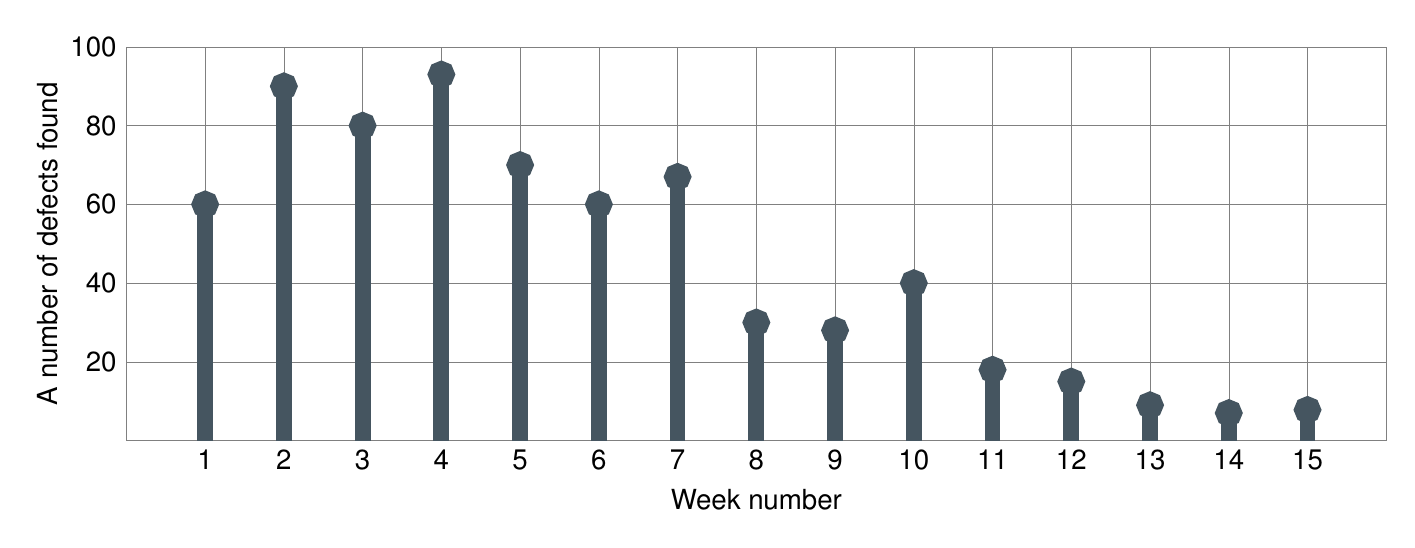
\begin{tikzpicture}
        \draw [help lines] (0,0) grid (16,5);
        \node [rotate=90, anchor=south] at (-0.75,2.5) {A number of defects found};
        \node [anchor=north] at (8,-0.5) {Week number};
        \foreach \y in {20, 40, 60, 80, 100} {\node [anchor=east] at ($\y*(0,0.05)$) {\y};};
        \foreach \x in {1, ..., 15} {\node [anchor=north] at ($\x*(1,0)$) {\x};};
        \draw [ycomb, mark=*, line width=0.2cm, color=tpcGrey] plot coordinates {
            % 1-Y means 20 changes
            (1,3)
            (2,4.5)
            (3,4)
            (4,4.65)
            (5,3.5)
            (6,3)
            (7,3.35)
            (8,1.5)
            (9,1.4)
            (10,2)
            (11,0.9)
            (12,0.75)
            (13,0.45)
            (14,0.35)
            (15,0.39)
        };
    \end{tikzpicture}
};
}

    \enru{
        During the project lifecycle, the customer took
        an active participation in discussions about system
        functionality with the system analyst, programmers, and testers.
    }{
        Во время всего проекта заказчик принимал активное участие
        в обсуждении функциональности ситемы, вместе с аналитиком, программистами
        и тестерами.
    }

    \enru{
        The first version of the system was delivered to the customer
        and manual testers in nine days after the project began.
        It was a workable software product, with very limited
        functionality implemented. During the next 16 weeks, the engineers
        made over 8000 alterations (check-ins), releasing new
        versions 10 to 20 times a day.
        We used \href{http://www.fazend.com}{fazend.com},
        a hosted continuous integration platform developed and maintained by our team.
    }{
        Первая версия системы была представлена заказчику и тестерам
        на девятый день (!) после старта проекта. Это был полностью рабочий
        продукт, в ограниченной функциональностью. В течение следующих
        16-ти недель инженеры сделали более восьми тысяч изменений в этом продукте,
        выдавая новую версию 10-20 раз в день. Для автоматизации этого процесса мы использовали
        \href{http://www.fazend.com}{fazend.com} --- систему собственной разработки.
    }

    \parpic(9em,7em)(-11em,6em){%
% Copyright (c) 2008, TechnoPark Corp., Florida, USA
% All rights reserved. THIS IS PRIVATE DOCUMENTATION.
%
% Redistribution and use in source and binary forms, with or without modification, are PROHIBITED
% without prior written permission from the author. This product may NOT be used anywhere
% and on any computer except the server platform of TechnoPark Corp. located at
% www.technoparkcorp.com. If you received this code occacionally and without intent to use
% it, please report this incident to the author}{email: privacy@technoparkcorp.com or
%}{mail: 568 Ninth Street South 202 Naples, Florida 34102, the United States of America,
% tel. +1 (239) 243 0206, fax +1 (239) 236-0738.
%
% @version $Id$
%
\tikz \node [scale=0.5] {
    \begin{tikzpicture}
        \newcommand{\cell}[4]{
            \node[regular polygon, regular polygon sides=6, minimum size=1cm, draw, inner sep=0cm, fill=#4]
            at ($#1*(0.75,0) + #2*(0,0.866) + #3*(0,0.433)$) {};
        }
        % empty
        \node [] at (0,0) (start) {
            \begin{tikzpicture}
            \cell{2}{-1}{0}{tpcLightGrey}\cell{2}{0}{0}{tpcLightGrey}\cell{2}{1}{0}{tpcLightGrey}
            \cell{1}{-2}{1}{tpcLightGrey}\cell{1}{-1}{1}{tpcLightGrey}\cell{1}{0}{1}{tpcLightGrey}\cell{1}{1}{1}{tpcLightGrey}
            \cell{0}{-2}{0}{tpcLightGrey}\cell{0}{-1}{0}{tpcLightGrey}\cell{0}{0}{0}{tpcLightGrey}\cell{0}{1}{0}{tpcLightGrey}\cell{0}{2}{0}{tpcLightGrey}
            \cell{-1}{-2}{1}{tpcLightGrey}\cell{-1}{-1}{1}{tpcLightGrey}\cell{-1}{0}{1}{tpcLightGrey}\cell{-1}{1}{1}{tpcLightGrey}
            \cell{-2}{-1}{0}{tpcLightGrey}\cell{-2}{0}{0}{tpcLightGrey}\cell{-2}{1}{0}{tpcLightGrey}
            \end{tikzpicture}
        };
        % partly filled
        \node [] at (5,0) (partly) {
            \begin{tikzpicture}
            \cell{2}{-1}{0}{tpcLightGrey}\cell{2}{0}{0}{tpcLightGrey}\cell{2}{1}{0}{tpcLightGrey}
            \cell{1}{-2}{1}{tpcLightGrey}\cell{1}{-1}{1}{tpcLightGrey}\cell{1}{0}{1}{tpcLightGrey}\cell{1}{1}{1}{tpcLightGrey}
            \cell{0}{-2}{0}{tpcLightGrey}\cell{0}{-1}{0}{tpcBlue}\cell{0}{0}{0}{tpcLightGrey}\cell{0}{1}{0}{tpcLightGrey}\cell{0}{2}{0}{tpcLightGrey}
            \cell{-1}{-2}{1}{tpcBlue}\cell{-1}{-1}{1}{tpcBlue}\cell{-1}{0}{1}{tpcLightGrey}\cell{-1}{1}{1}{tpcBlue}
            \cell{-2}{-1}{0}{tpcLightGrey}\cell{-2}{0}{0}{tpcLightGrey}\cell{-2}{1}{0}{tpcLightGrey}
            \end{tikzpicture}
        };
        % finished
        \node [] at (12,0) (finish) {
            \begin{tikzpicture}
            \cell{2}{-1}{0}{tpcBlue}\cell{2}{0}{0}{tpcBlue}\cell{2}{1}{0}{tpcBlue}
            \cell{1}{-2}{1}{tpcBlue}\cell{1}{-1}{1}{tpcBlue}\cell{1}{0}{1}{tpcLightGrey}\cell{1}{1}{1}{tpcBlue}
            \cell{0}{-2}{0}{tpcBlue}\cell{0}{-1}{0}{tpcBlue}\cell{0}{0}{0}{tpcBlue}\cell{0}{1}{0}{tpcBlue}\cell{0}{2}{0}{tpcBlue}
            \cell{-1}{-2}{1}{tpcBlue}\cell{-1}{-1}{1}{tpcBlue}\cell{-1}{0}{1}{tpcBlue}\cell{-1}{1}{1}{tpcBlue}
            \cell{-2}{-1}{0}{tpcBlue}\cell{-2}{0}{0}{tpcLightGrey}\cell{-2}{1}{0}{tpcBlue}
            \end{tikzpicture}
        };
        \draw [very thick, ->] (start) -- (partly);
        \draw [very thick, ->] (partly) -- node [midway, fill=white] {...} (finish);
    \end{tikzpicture}
};
}

    \enru{
        Empowered with \href{http://www.fazend.com/a/2010-03-PDD.html}{Puzzle Driven Development} paradigm,
        the team constructed the software as a puzzle mosaic. Every
        day we made many visible and tangible micro-steps,
        continuously approaching
        the final goal.
    }{
        Благодаря уникальной концепции \href{http://www.fazend.com/a/2010-03-PDD.html}{Puzzle Driven Development}
        команда создавала проект как мозаику. Каждый день
        мы делали видимый и ощутимый шаг вперед к конечной цели.
    }

    \enru{
        The deployment engineer was responsible for keeping the source code
        consistent and robust from day one. At the end of the
        project, the system included 29000 lines of code extensively
        documented and covered by unit tests for 85\%.
    }{
        Инженер по доставке был ответственен за целостность и качество
        исходного кода, начиная с первого дня проекта. В конце проекта
        мы получили 29 тысяч строк кода тщательно документированных и
        покрытых тестами на 85\% (!).
    }

    \enru{
        The quality of product was planned and controlled by means
        of pro-active bugs classification and enumeration, as originally suggested by~\citet{myers04}.
        We focused our testers on the forecasted amount of bugs we
        were going to fix in the product.
    }{
        Качество продукта планировалось и контролировалось при помощи
        активной классификации и нумерации дефектов, как предложил~\citet{myers04}.
        Мы ориентировали наших тестеров на ожидаемое число дефектов,
        которое требовалось обнаружить в продукте и затем устранить.
    }

    \enru{
        According to the signed contracts the testers were paid for
        the bugs found and documented, and they showed outstanding results.
        There were 700 bugs registered of different severities. 97\% of them
        were fixed before the end of the project, and the product was delivered on time and on budget, with
        all specified features.
    }{
        Согласно контрактам, тестеры получали оплату за найденные
        и задокументированные дефекты, и они показали отличные результаты.
        Всего было зарегистрировано более 700 дефектов разной сложности.
        97\% из них было устранено до завершения проекта.
        Продукт был создан вовремя и в рамках бюджета. Весь запланированный
        функционал был реализован.
    }




\phantomsection
\addcontentsline{toc}{section}{\enru{The Next Step}{Следующий Шаг}}
\section*{\enru{The Next Step}{Следующий Шаг}}

    \enru{
        At TechnoPark Corp., we keep researching and developing
        new processes and ways to develop software. There are a number of
        academic and industry papers we have produced during the last
        two years that emphasize
        certain aspects of our achievements, mostly by
        \cite{valid09,conflicts10,mensura09}.
    }{
        В течение последних двух лет было несколько публикаций,
        подчеркивающих некоторые формальные аспекты наших достижений, в том числе
        \cite{valid09,conflicts10,mensura09}. Исследования и разработки продолжаются.
    }

    \enru{
        We look forward to a new software development project with you that uses
        the XDSD methodology.
        For more information or to setup a meeting, please call us today at:~(239)~935~5429.
    }
    {
        Мы предлагаем выполнить с нами
        проект с использованием этой новой
        открытой методологии и нашей уникальной ее реализации.
    }


\appendix
\clearpage
\twocolumn
\phantomsection
\addcontentsline{toc}{section}{\enru{References}{Первоисточники}}
\renewcommand{\bibsection}{\enru{References}{Первоисточники}}
    \bibliographystyle{apalike}
    \bibliography{../main}

\end{document}
